\documentclass[aspectratio=169]{beamer}

% Theme settings
\usetheme{Madrid}
\usecolortheme{beaver}
\setbeamertemplate{navigation symbols}{}

% Packages
\usepackage{tikz}
\usepackage{booktabs}
\usepackage{amsmath}
\usepackage{pgfplots}
\pgfplotsset{compat=1.18}

% Meta information
\title{Unit 4: The Financial Sector}
\subtitle{Money, Banking, and Monetary Policy}
\author{Doğukan Günkördü}
\date{\today}

\begin{document}

% Title Slide
\begin{frame}
    \titlepage
\end{frame}

% Table of Contents
\begin{frame}{Outline}
    \tableofcontents
\end{frame}

% ==========================================
% SECTION 1: FINANCIAL ASSETS
% ==========================================
\section{Financial Assets}

\begin{frame}{Financial Assets: Key Concepts}
    \begin{itemize}
        \item \textbf{Financial Asset:} A paper claim that entitles the buyer to future income from the seller.
        \item \textbf{Liquidity:} How easily an asset can be converted into cash without loss of purchasing power.
        \item \textbf{Types of Assets:}
        \begin{itemize}
            \item \textbf{Money:} The most liquid asset (currency, checking accounts).
            \item \textbf{Stocks (Equity):} Ownership share in a corporation. High risk, potential for high return.
            \item \textbf{Bonds (Debt):} A loan to a government or corporation. The borrower pays interest and repays the principal at maturity.
        \end{itemize}
    \end{itemize}
\end{frame}

\begin{frame}{Bonds: Price vs. Yield}
    \begin{alertblock}{Crucial Relationship}
        Bond Prices and Interest Rates have an \textbf{inverse} relationship.
    \end{alertblock}
    
    \vspace{0.5cm}
    \begin{itemize}
        \item A bond pays a fixed coupon payment.
        \item If new interest rates in the economy \textbf{rise}, existing bonds paying lower rates become less desirable $\rightarrow$ their price \textbf{falls}.
        \item If new interest rates \textbf{fall}, existing bonds paying higher rates become more valuable $\rightarrow$ their price \textbf{rises}.
    \end{itemize}
\end{frame}

% ==========================================
% SECTION 2: NOMINAL VS REAL INTEREST RATES
% ==========================================
\section{Nominal vs. Real Interest Rates}

\begin{frame}{Nominal vs. Real Interest Rates}
    \begin{itemize}
        \item \textbf{Nominal Interest Rate ($i$):} The rate of interest paid for a loan, unadjusted for inflation. It is the price paid for the use of money.
        \item \textbf{Real Interest Rate ($r$):} The nominal rate adjusted for inflation. It represents the true cost of borrowing and the true payoff for lending.
    \end{itemize}

    \begin{block}{The Fisher Equation}
        \[ \text{Real Interest Rate} \approx \text{Nominal Interest Rate} - \text{Inflation Rate} \]
        \[ r = i - \pi \]
    \end{block}
    
    \begin{itemize}
        \item \textit{Example:} If the bank charges 7\% (nominal) and inflation is 2\%, the real cost of borrowing is 5\%.
    \end{itemize}
\end{frame}

% ==========================================
% SECTION 3: DEFINITION OF MONEY
% ==========================================
\section{Definition and Measurement of Money}

\begin{frame}{The Functions of Money}
    Money is anything society generally accepts in payment for goods and services.
    
    \vspace{0.5cm}
    \begin{enumerate}
        \item \textbf{Medium of Exchange:}
        \begin{itemize}
            \item Used to buy goods/services.
            \item Eliminates the "double coincidence of wants" required in barter.
        \end{itemize}
        \item \textbf{Unit of Account:}
        \begin{itemize}
            \item A measurement of value (like inches or degrees).
            \item Allows us to compare prices (e.g., a car costs \$20,000, a soda costs \$2).
        \end{itemize}
        \item \textbf{Store of Value:}
        \begin{itemize}
            \item Allows purchasing power to be saved for the future.
            \item Inflation erodes this function.
        \end{itemize}
    \end{enumerate}
\end{frame}

\begin{frame}{Types of Money \& The Money Supply}
    \begin{itemize}
        \item \textbf{Fiat Money:} Money that has value because the government says it is legal tender (no intrinsic value like gold).
    \end{itemize}

    \vspace{0.3cm}
    \textbf{Measuring the Money Supply (Liquidity):}
    \begin{itemize}
        \item \textbf{M1 (High Liquidity):}
        \begin{itemize}
            \item Currency in circulation.
            \item Demand deposits (Checking accounts).
            \item Other liquid deposits (Savings accounts - \textit{updated Fed definition}).
        \end{itemize}
        \item \textbf{M2 (M1 + Near Monies):}
        \begin{itemize}
            \item Everything in M1.
            \item Small time deposits (CDs).
            \item Retail money market funds.
        \end{itemize}
    \end{itemize}
\end{frame}

% ==========================================
% SECTION 4: BANKING & MONEY EXPANSION
% ==========================================
\section{Banking and Money Expansion}

\begin{frame}{Fractional Reserve Banking}
    \begin{itemize}
        \item \textbf{Fractional Reserve System:} Banks keep only a fraction of deposits as reserves and loan out the rest.
        \item \textbf{Reserves:}
        \begin{itemize}
            \item \textbf{Required Reserves:} The portion of deposits the Fed requires banks to hold (determined by the Reserve Ratio).
            \item \textbf{Excess Reserves:} Reserves held above the requirement. These can be loaned out.
        \end{itemize}
    \end{itemize}
    
    \begin{block}{Calculations}
        \[ \text{Total Reserves} = \text{Required} + \text{Excess} \]
    \end{block}
\end{frame}

\begin{frame}{The Money Multiplier}
    When banks loan out excess reserves, money is created (deposited in another bank, creating new reserves, allowing new loans).

    \begin{block}{The Money Multiplier Formula}
        \[ \text{Money Multiplier} = \frac{1}{\text{Reserve Requirement Ratio}} \]
    \end{block}

    \begin{itemize}
        \item \textbf{Maximum Change in Money Supply:}
        \[ \Delta \text{Money Supply} = \text{Multiplier} \times \Delta \text{Excess Reserves} \]
    \end{itemize}
    
    \textit{Note: "Cash drain" (people holding cash) or banks holding excess reserves will reduce the actual multiplier effect.}
\end{frame}

% ==========================================
% SECTION 5: THE MONEY MARKET
% ==========================================
\section{The Money Market}

\begin{frame}{The Money Market Graph}
    The interaction of the demand for money and the supply of money determines the \textbf{Nominal Interest Rate}.

    \begin{columns}
        \column{0.5\textwidth}
        \begin{itemize}
            \item \textbf{Money Demand ($M_d$):} Downward sloping.
            \begin{itemize}
                \item Transaction demand (buying stuff).
                \item Asset demand (holding cash vs. bonds).
            \end{itemize}
            \item \textbf{Money Supply ($M_s$):} Vertical.
            \begin{itemize}
                \item Determined independently by the Fed.
            \end{itemize}
        \end{itemize}

        \column{0.5\textwidth}
        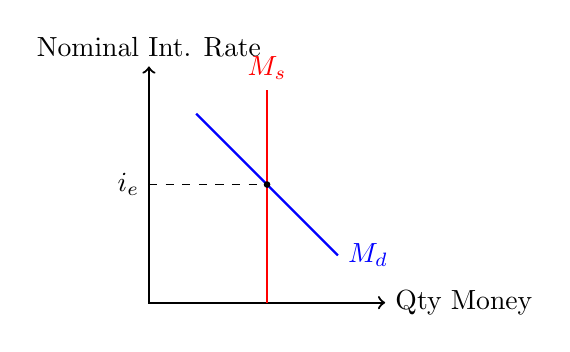
\begin{tikzpicture}[scale=0.6]
            \draw[thick, <->] (0,5) node[above]{Nominal Int. Rate} -- (0,0) -- (5,0) node[right]{Qty Money};
            % Md
            \draw[thick, blue] (1,4) -- (4,1) node[right]{$M_d$};
            % Ms
            \draw[thick, red] (2.5,0) -- (2.5,4.5) node[above]{$M_s$};
            % Equilibrium
            \draw[dashed] (0,2.5) node[left]{$i_e$} -- (2.5,2.5);
            \fill (2.5,2.5) circle (2pt);
        \end{tikzpicture}
    \end{columns}
\end{frame}

\begin{frame}{Shifting the Money Market}
    \begin{columns}
        \column{0.5\textwidth}
        \textbf{Shifters of Money Demand:}
        \begin{enumerate}
            \item \textbf{Price Level:} Prices $\uparrow$, need more cash $\rightarrow$ $M_d$ shifts right.
            \item \textbf{Income (Real GDP):} Income $\uparrow$, more transactions $\rightarrow$ $M_d$ shifts right.
            \item \textbf{Technology:} Credit cards/Venmo make cash less needed $\rightarrow$ $M_d$ shifts left.
        \end{enumerate}

        \column{0.5\textwidth}
        \textbf{Shifters of Money Supply:}
        \begin{enumerate}
            \item \textbf{Monetary Policy:}
            \begin{itemize}
                \item Fed buys bonds $\rightarrow$ $M_s$ shifts right (Rates $\downarrow$).
                \item Fed sells bonds $\rightarrow$ $M_s$ shifts left (Rates $\uparrow$).
            \end{itemize}
        \end{enumerate}
    \end{columns}
\end{frame}

% ==========================================
% SECTION 6: MONETARY POLICY
% ==========================================
\section{Monetary Policy}

\begin{frame}{Tools of the Federal Reserve}
    The Fed manages the money supply to achieve \textbf{dual mandates}: Price Stability and Maximum Employment.

    \begin{enumerate}
        \item \textbf{Reserve Requirement:}
        \begin{itemize}
            \item Lowering it creates excess reserves $\rightarrow$ Money Supply $\uparrow$.
        \end{itemize}
        \item \textbf{Discount Rate:}
        \begin{itemize}
            \item The rate the Fed charges banks for short-term loans.
            \item Lower rate encourages borrowing $\rightarrow$ Money Supply $\uparrow$.
        \end{itemize}
        \item \textbf{Open Market Operations (OMO):}
        \begin{itemize}
            \item Buying/Selling government bonds.
            \item \textbf{Buy Bonds = Big Bucks (Expansionary).}
            \item \textbf{Sell Bonds = Small Bucks (Contractionary).}
        \end{itemize}
        \item \textbf{Interest on Reserves (IOR):}
        \begin{itemize}
            \item Fed pays interest on bank reserves. Lower IOR encourages banks to lend $\rightarrow$ Money Supply $\uparrow$.
        \end{itemize}
    \end{enumerate}
\end{frame}

\begin{frame}{Expansionary vs. Contractionary Policy}
    \begin{table}[]
        \begin{tabular}{@{}p{3.5cm}p{4cm}p{4cm}@{}}
            \toprule
            \textbf{Policy} & \textbf{Action} & \textbf{Result} \\ \midrule
            \textbf{Expansionary} \newline (Recession) & Buy Bonds \newline Lower Disc. Rate \newline Lower Res. Req. \newline Lower IOR & $M_s \uparrow$ \newline Nom. Int. Rate $\downarrow$ \newline Investment $\uparrow$ \newline AD $\uparrow$ \\ \midrule
            \textbf{Contractionary} \newline (Inflation) & Sell Bonds \newline Raise Disc. Rate \newline Raise Res. Req. \newline Raise IOR & $M_s \downarrow$ \newline Nom. Int. Rate $\uparrow$ \newline Investment $\downarrow$ \newline AD $\downarrow$ \\ \bottomrule
        \end{tabular}
    \end{table}
\end{frame}

% ==========================================
% SECTION 7: LOANABLE FUNDS MARKET
% ==========================================
\section{The Market for Loanable Funds}

\begin{frame}{Loanable Funds Market Graph}
    This market connects Savers (Supply) and Borrowers (Demand). It determines the \textbf{Real Interest Rate}.

    \begin{columns}
        \column{0.5\textwidth}
        \begin{itemize}
            \item \textbf{Supply ($S_{LF}$):} Upward sloping.
            \begin{itemize}
                \item Household savings.
                \item Capital Inflows (foreign money).
            \end{itemize}
            \item \textbf{Demand ($D_{LF}$):} Downward sloping.
            \begin{itemize}
                \item Business Investment.
                \item Government borrowing (deficit spending).
            \end{itemize}
        \end{itemize}

        \column{0.5\textwidth}
        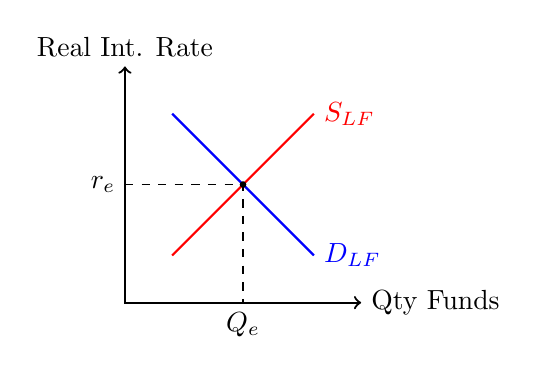
\begin{tikzpicture}[scale=0.6]
            \draw[thick, <->] (0,5) node[above]{Real Int. Rate} -- (0,0) -- (5,0) node[right]{Qty Funds};
            % Demand
            \draw[thick, blue] (1,4) -- (4,1) node[right]{$D_{LF}$};
            % Supply
            \draw[thick, red] (1,1) -- (4,4) node[right]{$S_{LF}$};
            % Equilibrium
            \draw[dashed] (0,2.5) node[left]{$r_e$} -- (2.5,2.5) -- (2.5,0) node[below]{$Q_e$};
            \fill (2.5,2.5) circle (2pt);
        \end{tikzpicture}
    \end{columns}
\end{frame}

\begin{frame}{Crowding Out}
    \textbf{Crowding Out} occurs when the government deficit spends.
    
    \vspace{0.3cm}
    \begin{enumerate}
        \item Government runs a deficit $\rightarrow$ must borrow money.
        \item Demand for Loanable Funds ($D_{LF}$) shifts \textbf{Right}.
        \item \textbf{Real Interest Rate rises.}
        \item Higher interest rates make it expensive for businesses to borrow.
        \item Private Investment ($I_g$) \textbf{decreases}.
    \end{enumerate}
    
    \vspace{0.3cm}
    \textit{Result: Government spending replaces (crowds out) private investment, potentially slowing long-run growth.}
\end{frame}

\end{document}
